\section{Experiments and Results} \label{sec:experimentsResults}

The performance of the torque and impedance controllers were assessed by experimental tests  both in terms of {\em transparency} and {\em haptic rendering} performance measures. 
The tests show how the torque controls behave in constant and varying desired torque tracking.
The first one is the transparency test in which the robot tries to keep the joint torque at zero Nm while the user is moving the exoskeleton.
The second test is the haptic rendering with a slanted flat surface with different simulated stiffness.
More details on each test are reported in the subsections below.
\par The implemented control laws (\ref{eq:JTCF1_control_law_uf_simple}), (\ref{JTFC2_control_law_final}) and (\ref{control_law_Kugi_2}) have been set using the model parameters. The proportional and derivative PD gains ($K_p$ and $K_d$) have been chosen to obtain a desired error dynamics, specifically the form that guarantees the minimum ITAE index. Notice that the control laws (\ref{eq:JTCF1_control_law_uf_simple}) and (\ref{JTFC2_control_law_final}) have two degrees of freedom, i.e. $K_p$ and $K_d$ can be independently chosen, whereas the control law (\ref{control_law_Kugi_2}) exhibits only one degree of freedom, thus the two control gains are linked and they are calculated as a function of the desired inertia $I_{\theta}$.

%%%%%%%%%%%%%%%%%%%%%%%%%%%%%%%%%%%%%%%%%%%%%%%%%%%%%%%%%%%%%%%%%%%%%%%%%%%%%%%%%%%%%%%%%%%%%%%%%%%%%%%%%%%%%%%%%%%%
%%%%%%%%%%%%%%%%%%%%%%%%%%%%%%%%%%%%%%%%%%%%%%%%%%%%%%%%%%%%%%%%%%%%%%%%%%%%%%%%%%%%%%%%%%%%%%%%%%%%%%%%%%%%%%%%%%%%
\subsection{Transparency} \label{subsec:transparency}

For the transparency test, 
a performance measurements was adopted based on multi-joint transparency as in \cite{just2018exoskeleton} were the pHRI torque on each joint has been analyzed.
More in detail, two kinds of trials have been done.
The first type of trial uses the JTFC1 control law described in the subsection \ref{subsec:JTFC1} in order to verify how much the dynamics compensations improve the desired torque tracking.
The second type of trials compare the three control laws and its aim is to understand how the terms of the controllers are related to the desired torque tracking.

The transparency tests were performed recruiting 10 healthy subjects (males, 8 right-handed) with a mean age: 30.9 $\pm$ 5.2 years. All  subjects were asked to sign a written informed consent for participating to the study.

The two transparency tests have a slightly difference: in the first trials the user moves  the exoskeleton wit no constraints, grabbing the end-effector handle (interaction forces are exerted only at the end-effector). Whereas, during the second transparency test, the user is linked with the exoskeleton at 2 anchor points at the  arm and the forearm (by grasping the end-effector handle).
An additional force sensor was mounted on the end-effector of the exoskeleton to measure the actual forces $\vects{F_h^*}$  applied by the user at the handle interface. 

\par  As transparency index we evaluated the mean absolute pHRI torque and the mean peak absolute pHRI torque as in \cite{just2018exoskeleton}. The measured end-effector forces provides only a qualitative index in the transparency test when a multi-contact interaction with the exoskeleton occurs. Conversely, the measured end effector norm force have been used to quantitative evaluate the controller performances during single-contact interactions.
%The reflected torques at the joint are calculated as $\vects{\tau_s^*}=\vects{J^T F_h^*}$ and then compared to the interaction torques estimated by the optimal observer.

\subsubsection{How dynamic compensation affects the transparency} \label{subsubsec:compensationAndTransparency}

In order to understand how the dynamic compensation affects the transparency the scheme of figure \ref{fig:fullstate} has been implemented using the JTFC1 control law plus the dynamics terms multiplied by $\alpha$, with $0 \leq \alpha \leq 1$.

In this test, the subject is asked to perform sinusoidal movements at each joint with a range of $10 ~ deg \simeq 0.2 ~ rad $ with a frequency of $0.5 ~ Hz$, thus similar acceleration are imprinted to the exoskeleton joint for both \textquotedblleft dynamic compensation\textquotedblright \ and \textquotedblleft no compensation conditions\textquotedblright.

The experimental results for torque tracking, with a desired torque $\vects{\tau_s^D=0}$, are shown for the second joint $J_2$ in \figurename \ \ref{fig:torque_validation}, that is the joint with the highest link inertia.  The control was set to follow his movement at zero-torque with (\figurename \ \ref{fig:torque_validation}, left) and without (\figurename \ \ref{fig:torque_validation}, right) dynamics compensation.
 
\par The upper plots show the joint position (black solid line), the central plots display the estimated acceleration (gray dashed line), to demonstrate the movements were similar in both cases. The lower plots represent the interaction torques estimated by the observer (gray dashed line) and measured by the force sensor (black solid line). Even if the estimated torques are similar in both cases, with dynamics compensation the actual interaction forces are lower, demonstrating that torque tracking is more precise and the user has to compensate less for the link dynamics.

%\begin{figure}[htb]
%	\centering
%	\subfigure[Without dynamics compensation]{ 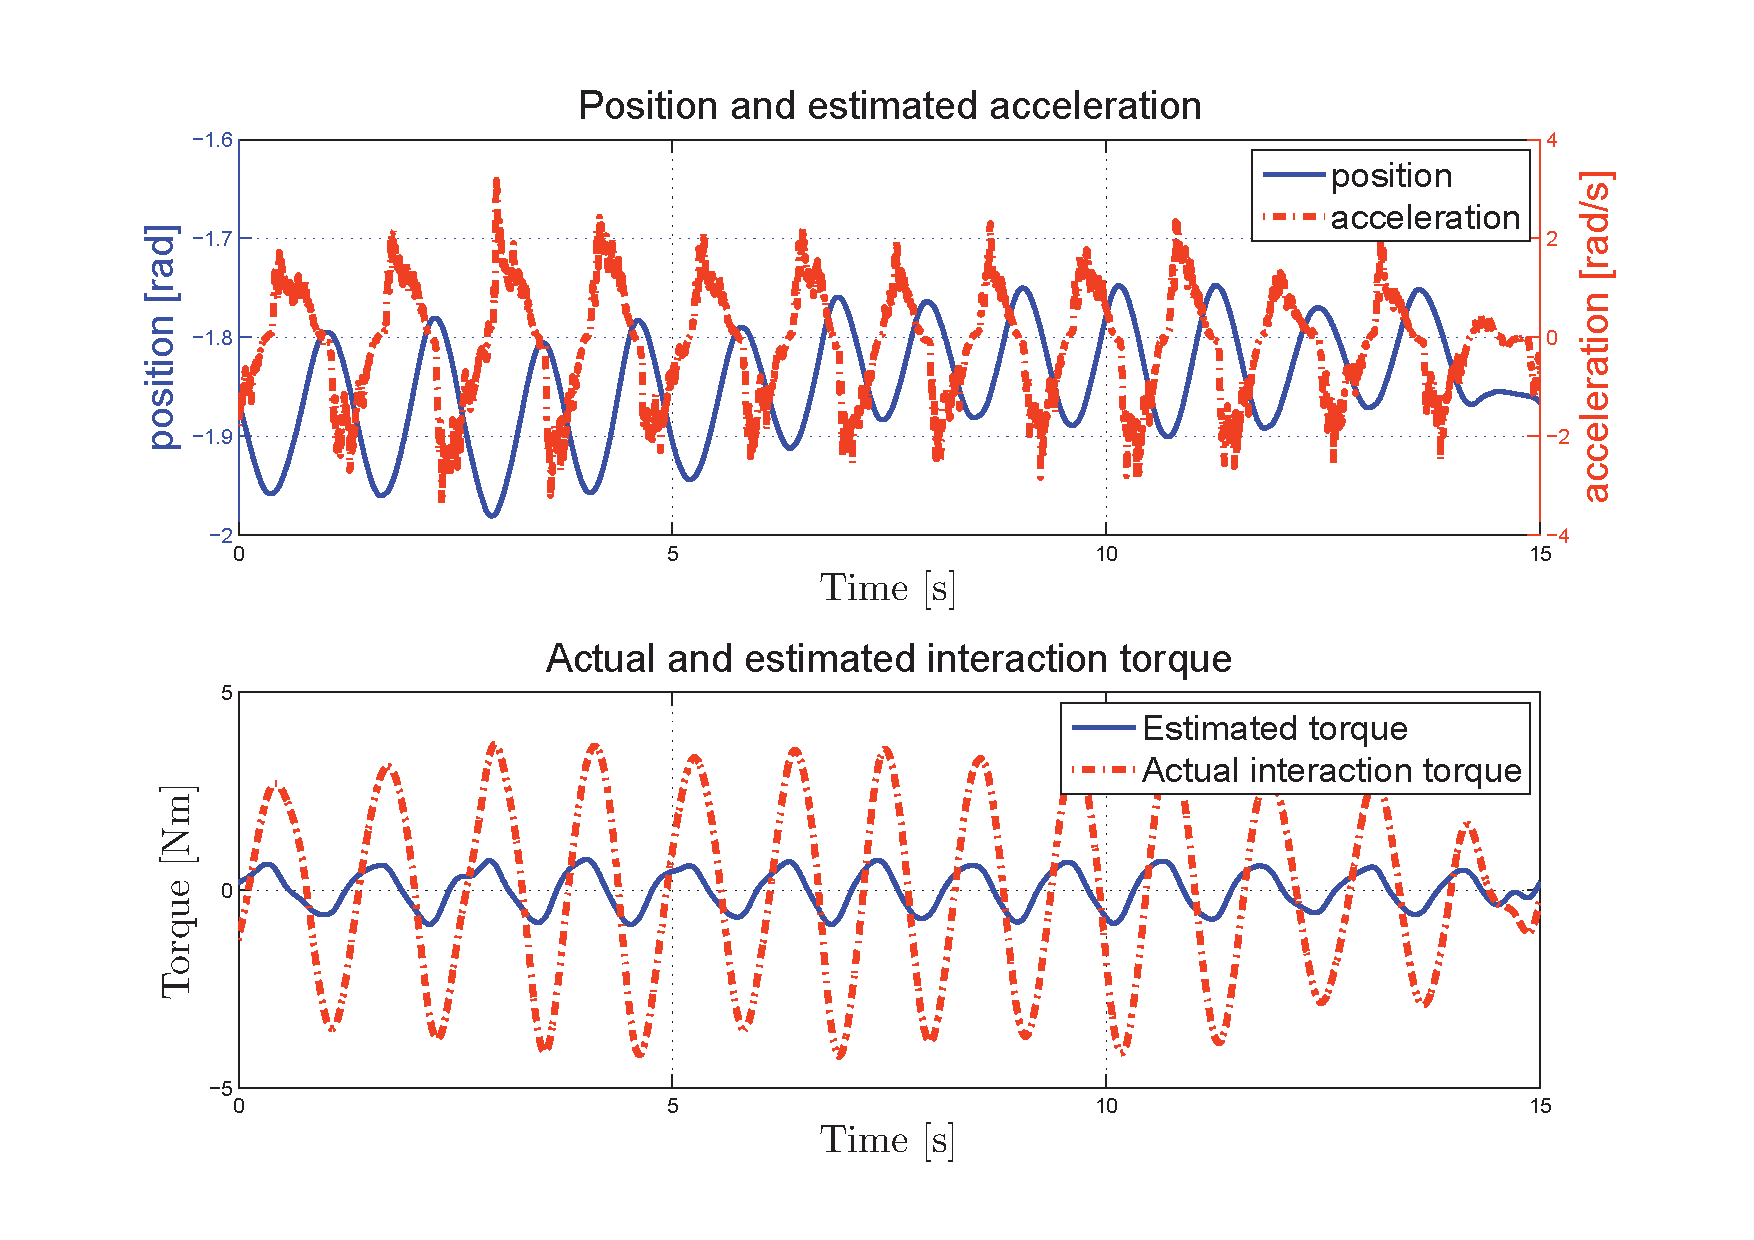
\includegraphics[width=1\columnwidth]{a_p_ts2_vs_ets2_nocomp.pdf}\label{fig:torque_validation_nocomp}}
%	\subfigure[With dynamics compensation]{  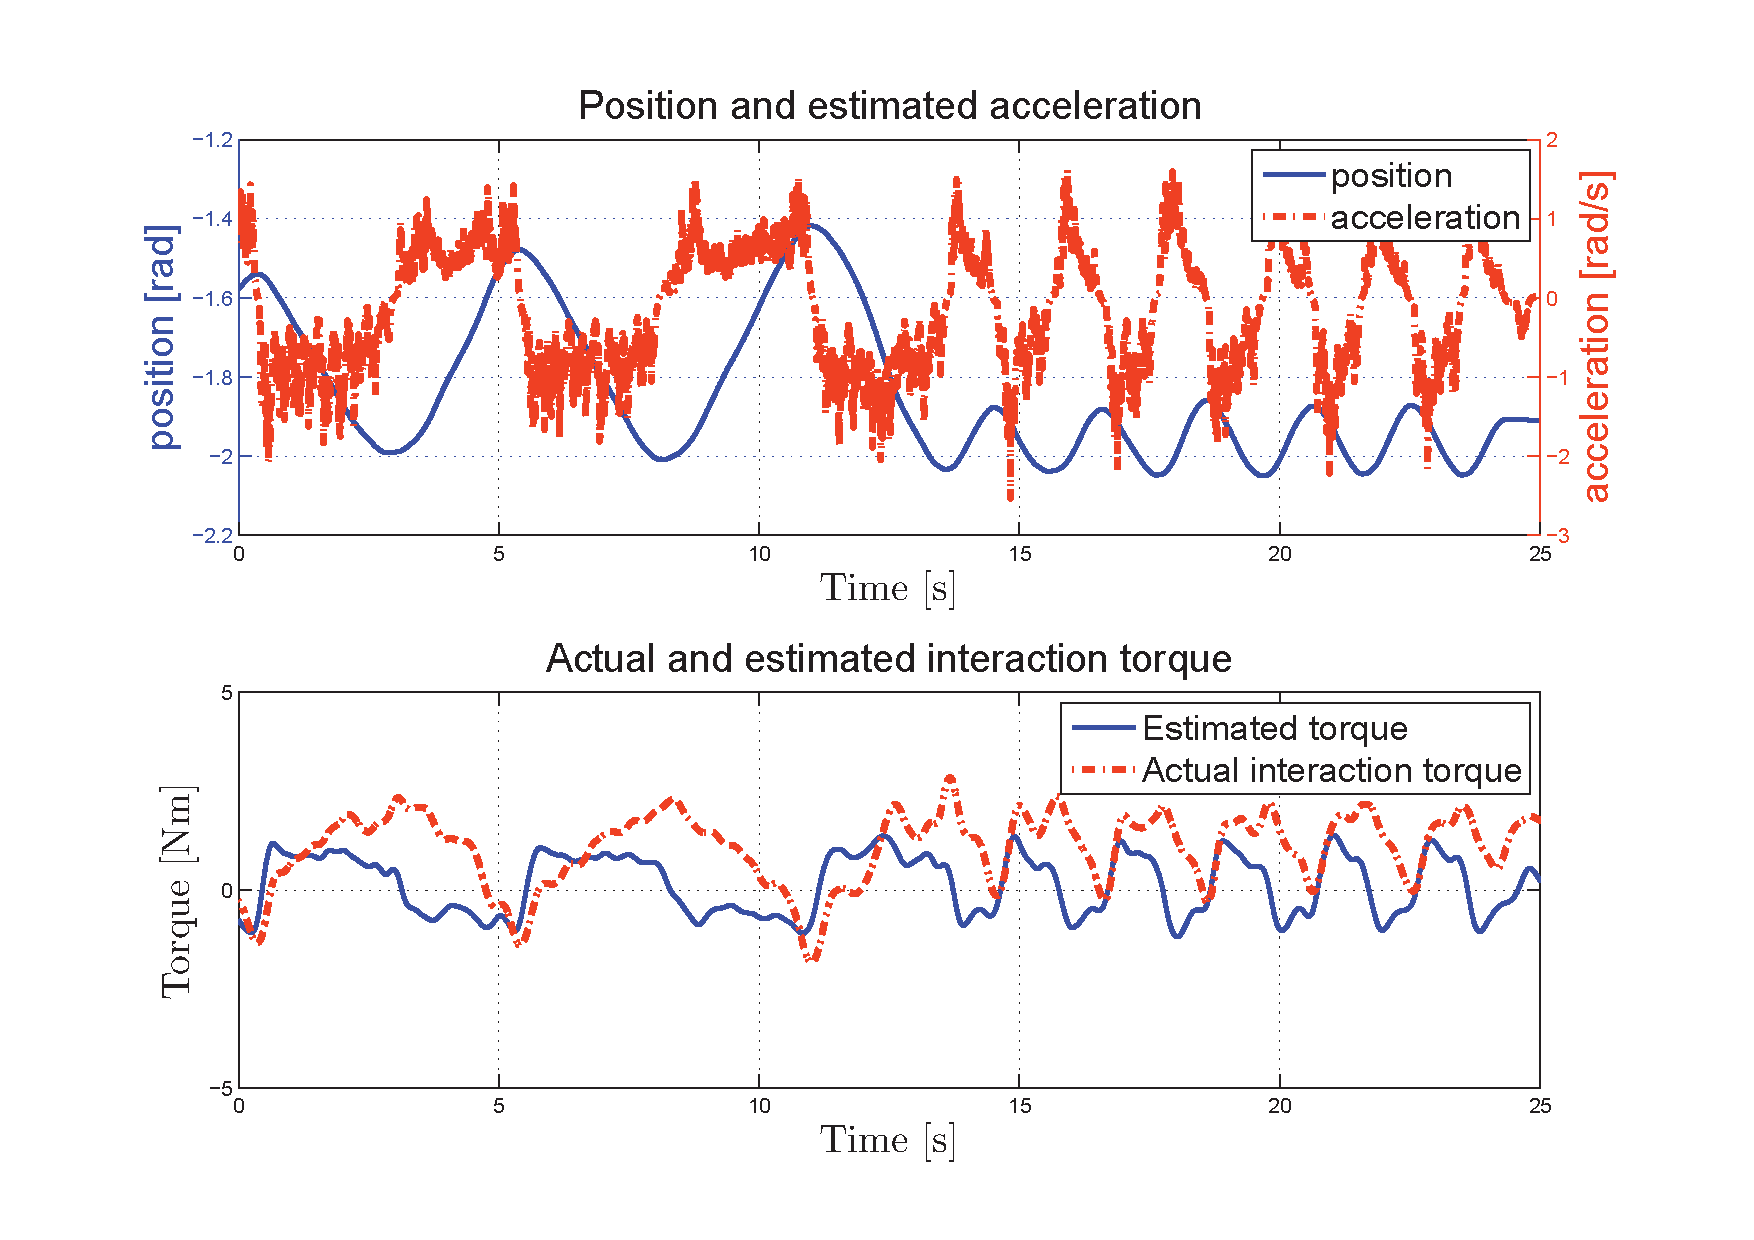
\includegraphics[width=1\columnwidth]{a_p_ts2_vs_ets2_comp.pdf}\label{fig:torque_validation_comp}}
%	\caption{Comparison between the measured torque $\tau_s$ and calculated torque by force sensor \hldoing{units of acc wrong, which joint??}}
%	\label{fig:torque_validation}
%\end{figure}

\begin{figure*}[htb]
	\centering
	\def\svgwidth{2\columnwidth}
	\begin{footnotesize}
		\input{imgRevised/dynamic_compens_vs_no_compens.pdf_tex}
	\end{footnotesize}
	\caption{Comparison between the estimated torque $\tau_s$ and the actual torque that is calculated by force sensor for joint $J_2$ (third row). Experiment was carried out providing dynamics compensation (left side) and without dynamics compensation (right side, in gray). For the two conditions, angular position and acceleration are reported in the first and second row respectively. Without dynamics compensations, the actual torques differs from the estimated ones resulting in a loss of transparency. }
	\label{fig:torque_validation}
\end{figure*}

\subsubsection{Comparison between the three torque controllers JTFC1, JTFC2 and JTFC3}

\begin{figure}[htb]
	\centering
	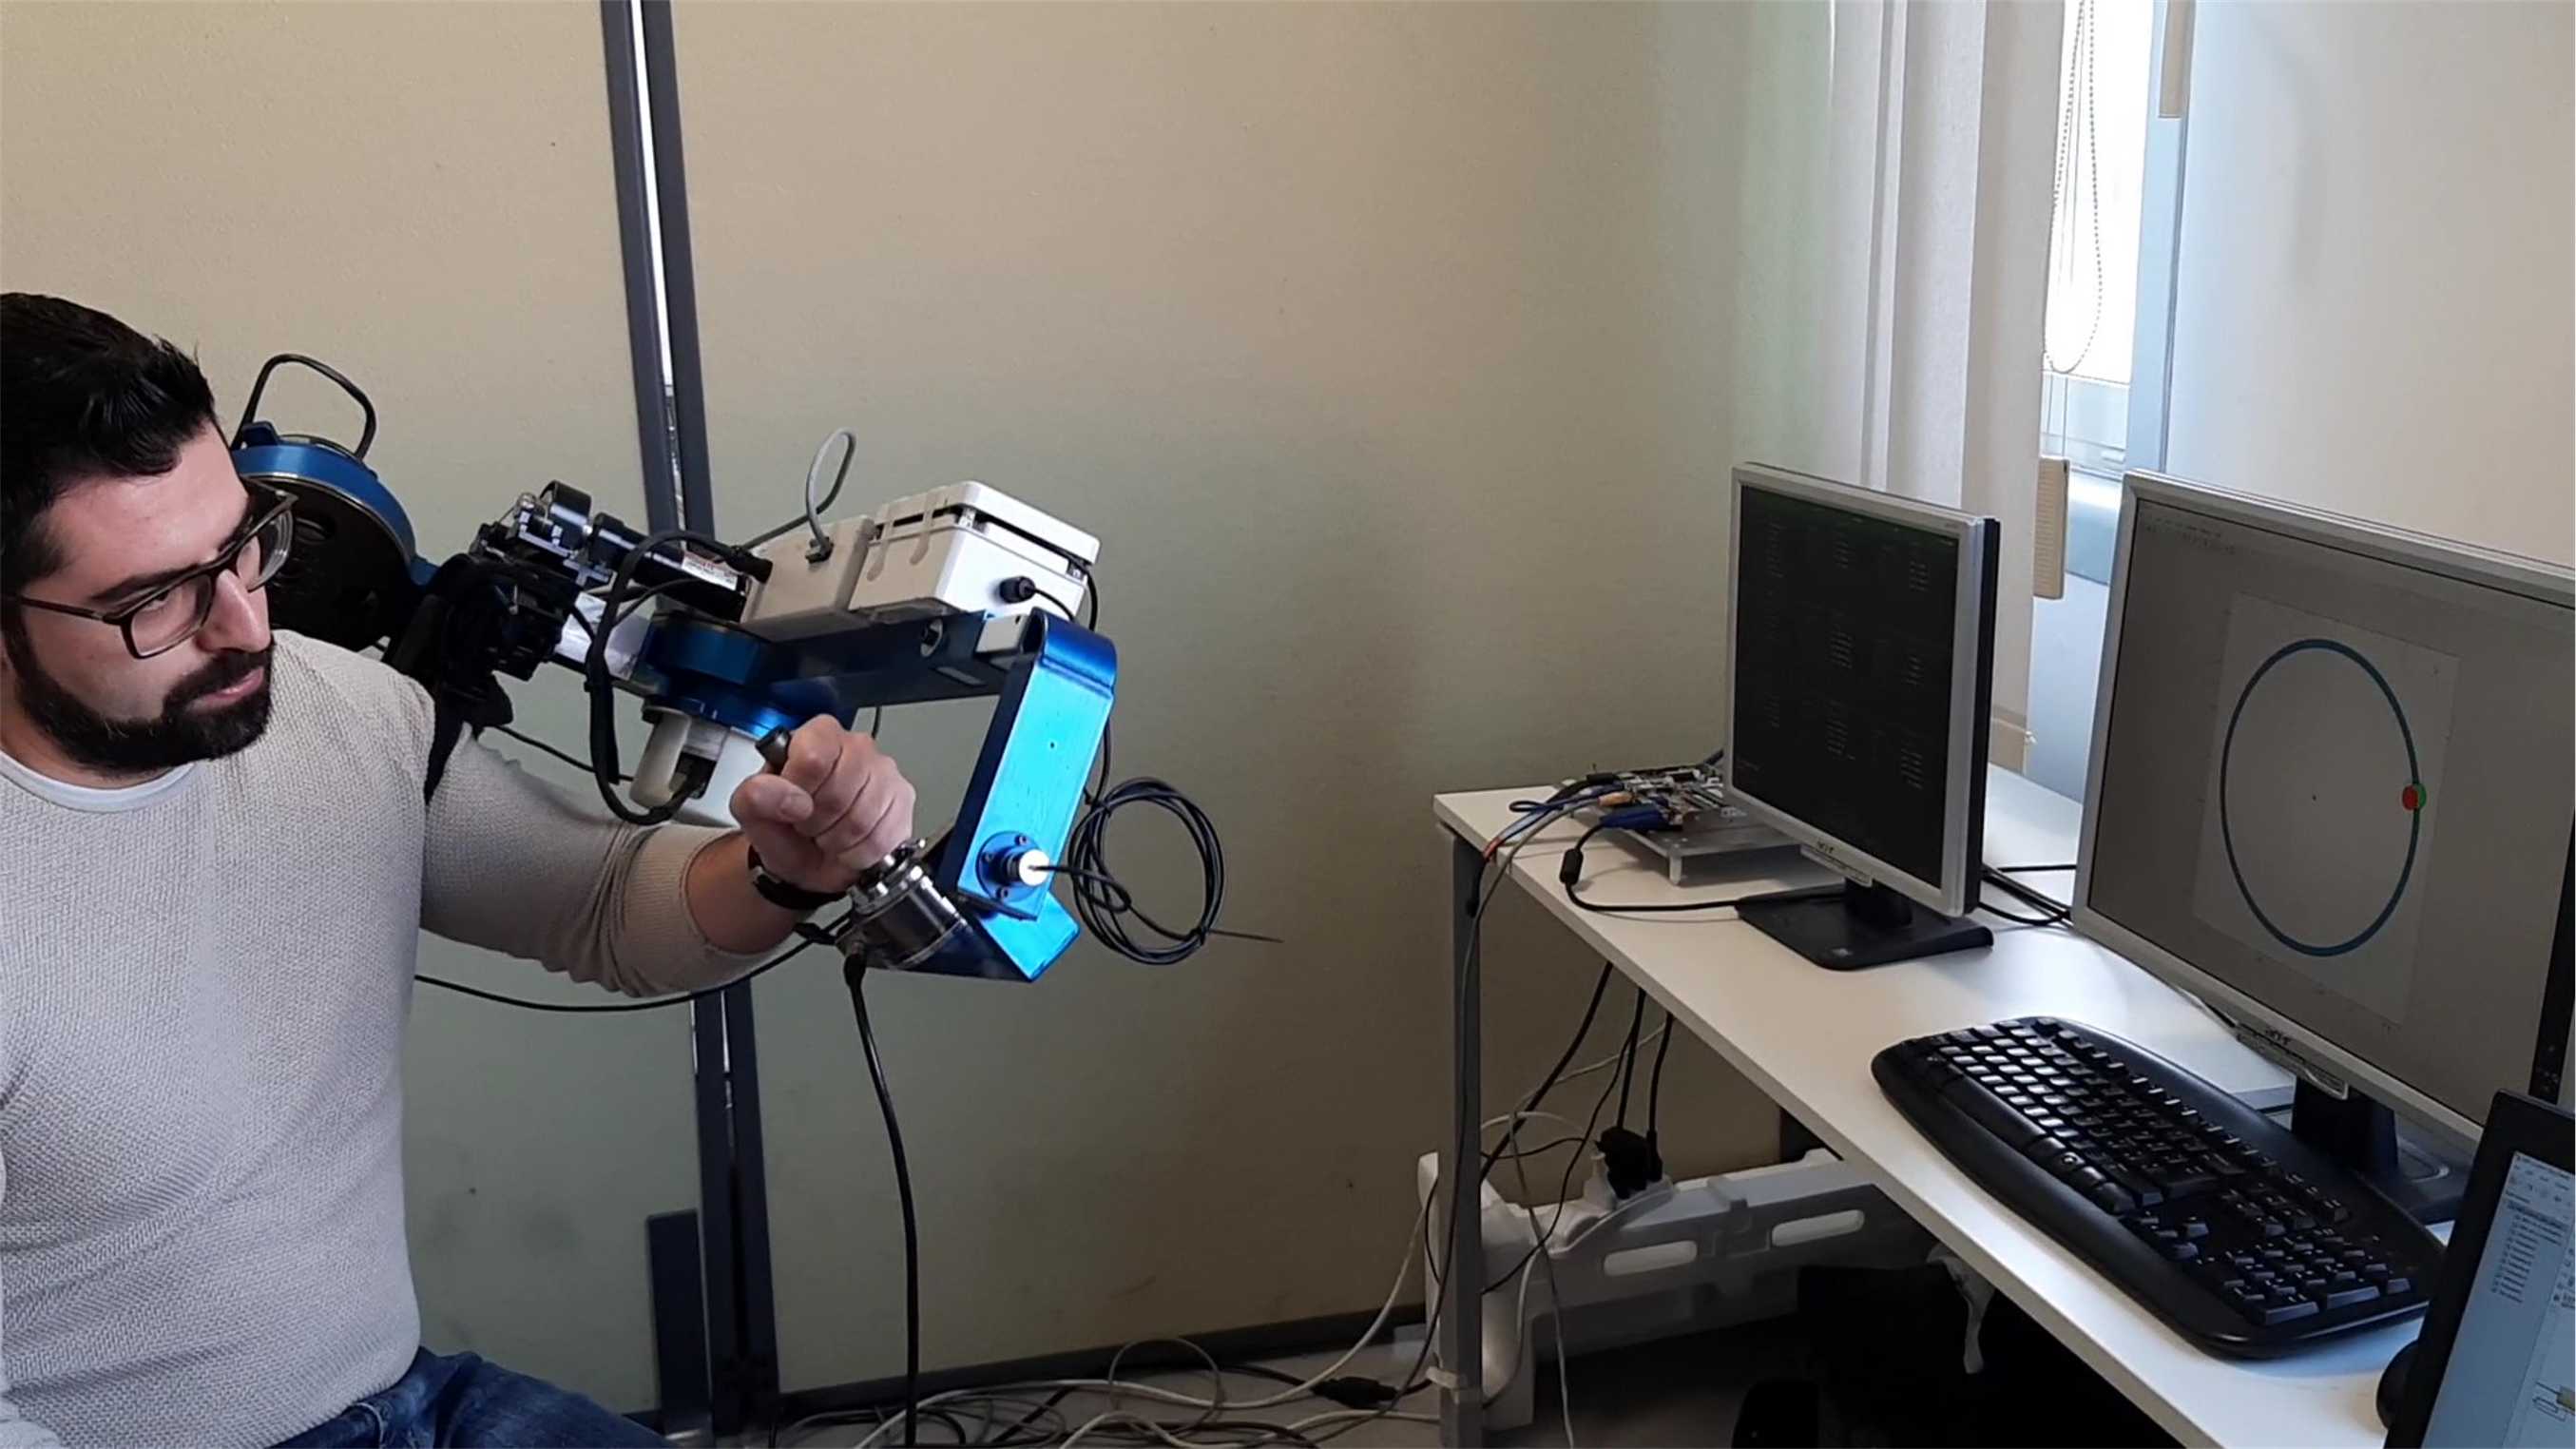
\includegraphics[width=1\columnwidth]{experiment_setup}
	\caption{Experimental setup of the transparency test. The user is linked to the exoskeleton at the shoulder level and at the end-effector (it grabs the handle).  The user's elbow and the exoskeleton's one enter in contact during the trial execution. The subject moved the exoskeleton performing a circular trajectory at constant angular speed which reference is shown on a screen.}
	\label{fig:experimentalSetup}
\end{figure}

For this kind of trials the three joint torque controls presented in the section \ref{sec:Full_state_feedback_controllers} were tested with a desired torque set to zero ($\vects{\tau_s^D=0}$).% as for the trials in the subsection \ref{subsubsec:compensationAndTransparency}. 
The tests were conducted as in \cite{just2018exoskeleton}: the participants were asked to track a reference point on a circular path, displayed on a screen, with the end-effector parallel to the coronal plane in front of them. Figure \ref{fig:experimentalSetup} shows a subject while performing the transparency task.
The diameter of the circle was equal to $0.3 ~ m$ and the center position was set to the subject's chest height to move in a typical activities of daily living workspace. Circles have been performed at two speed levels: slow ($45 ~ \frac{deg}{s}$) and fast ($90 ~ \frac{deg}{s}$) in accordance with \cite{just2018exoskeleton}. 10 repetitions for each speed level. 
Moreover, the sequence of the controllers was randomly assigned to each participant to mitigate potential order effects.


%\hldoing{adding a figure showing circle location}

%\hldoing{simulating test with two more subjects??.}
%Despite the user tried to track the desired trajectory, the executed ones and their speeds were someway influenced by the used torque control. The average speed at the end effector of the three controls are listed in the \tablename \ \ref{tab:transparencySpeeds}.
%
%\begin{table}[!t]
%	\renewcommand{\arraystretch}{1.3}
%	\caption{The natural frequency of the joints}
%	\label{tab:transparencySpeeds}
%	\centering
%	\begin{tabular}{|c|c|c|}
%		\hline
%		\bfseries Control & \bfseries Avg. speed [$m/s$] & \bfseries Std. dev. [$m/s$]\\
%		\hline\hline
%		JTFC1 & 0.4198 & 0.0810\\
%		\hline
%		JTFC2 & 0.4460 & 0.1374\\
%		\hline
%		JTFC3 & 0.3867 & 0.1213\\
%		\hline
%	\end{tabular}
%\end{table}
%\begin{table}[]
%	\renewcommand{\arraystretch}{1.3}
%	\caption{Mean and Std. Dev. of the e.e. speed in the transparency experiments}
%	\label{tab:transparencySpeeds}
%	\centering
%	\begin{tabular}{c c c}
%		\hline \hline
%		\bfseries Control & \bfseries Avg. speed [$m/s$] & \bfseries Std. dev. [$m/s$]\\
%		\hline
%		JTFC1 & 0.4198 & 0.0810\\
%		JTFC2 & 0.4460 & 0.1374\\
%		JTFC3 & 0.3867 & 0.1213\\
%		\hline \hline
%	\end{tabular}
%\end{table}
%
The comparative multi-joint transparency study is depicted in Fig. \ref{fig:transparencyJointErrors} whereas the real trajectories performed by a representative subject can be shown in the \figurename \ \ref{fig:traittorie3D}. 

\begin{figure}[htb]
	\centering
%	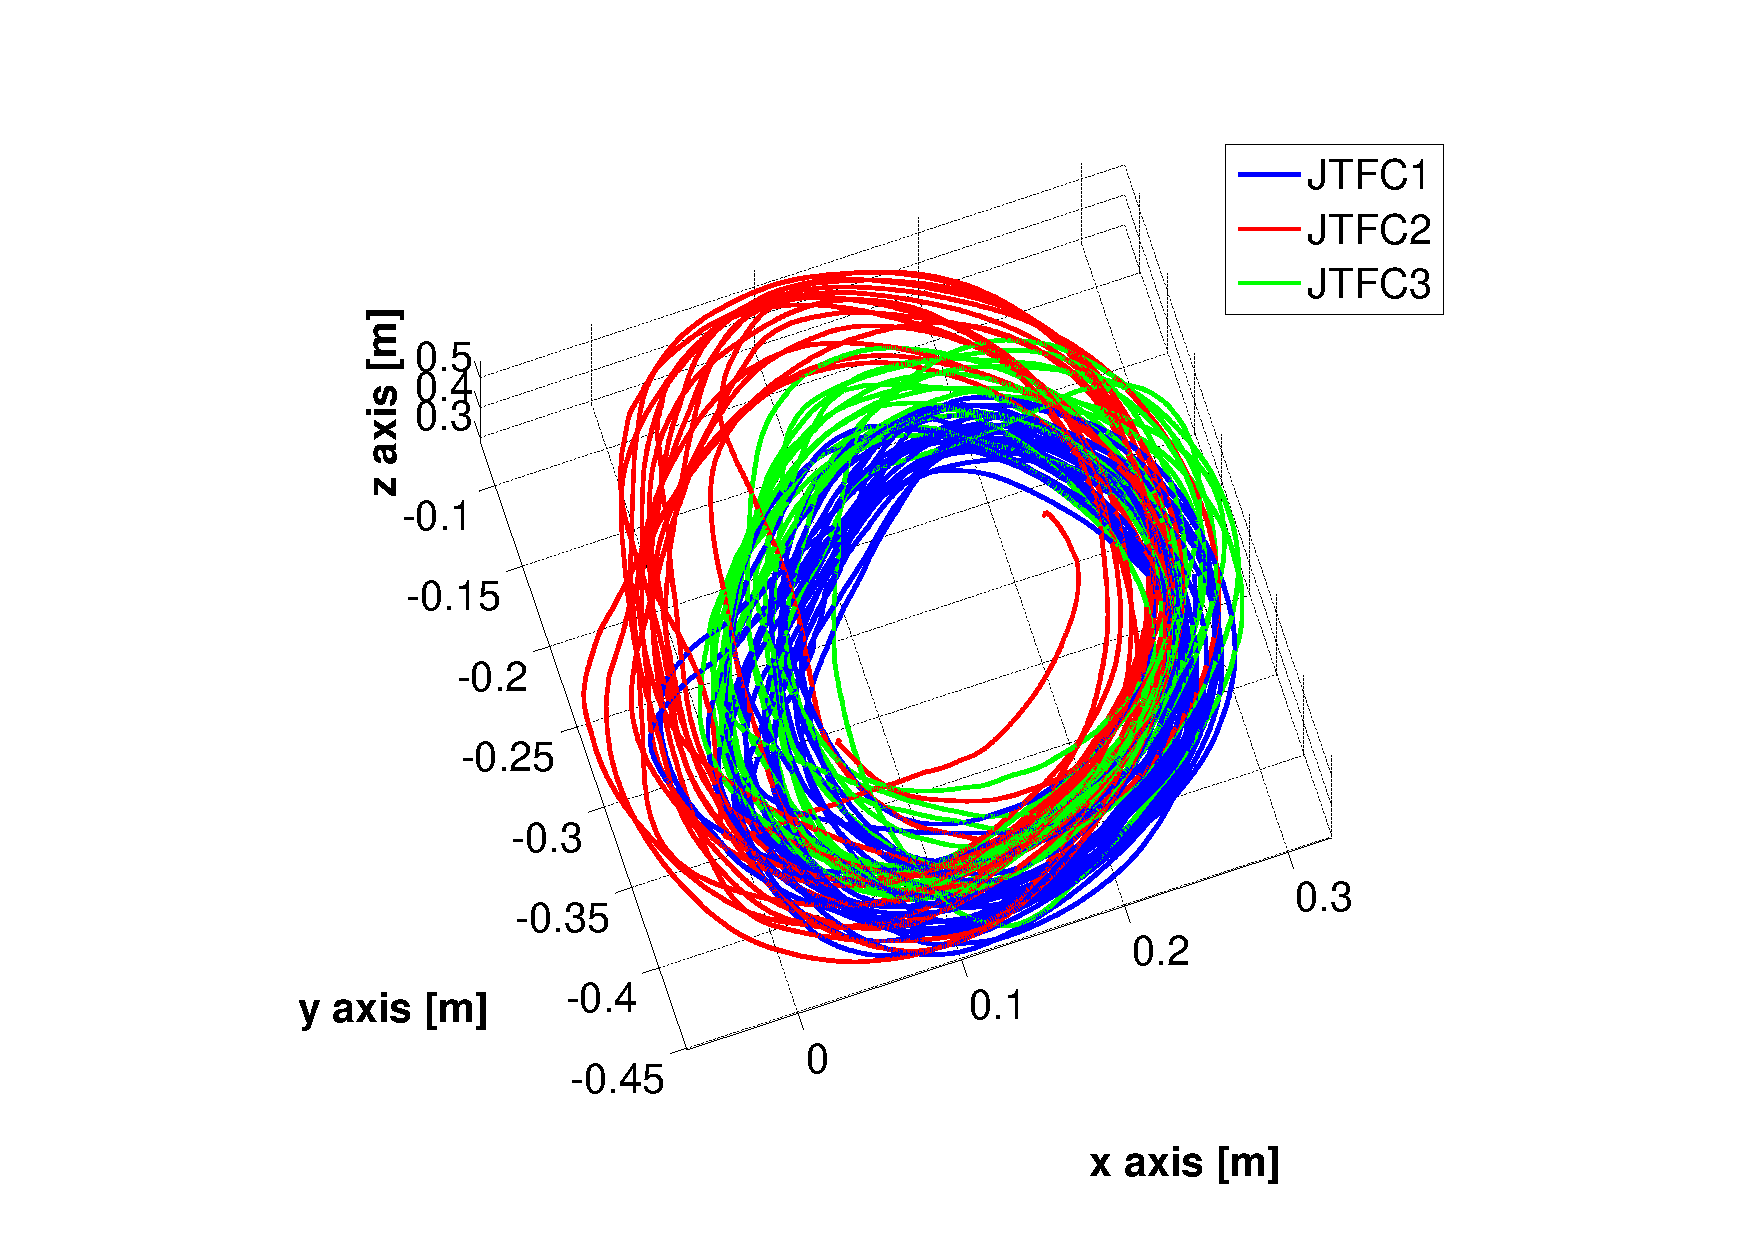
\includegraphics[width=0.99\columnwidth]{traiettorieCircolari2}
\def\svgwidth{0.95\columnwidth}
	\begin{footnotesize}
		\input{imgRevised/circles2.pdf_tex}
	\end{footnotesize}
	\caption{The trajectories performed during the transparency test using the three control laws in the slow (first row) and fast (second row) conditions.}
	\label{fig:traittorie3D}
\end{figure}

Fig. \ref{fig:transparencyJointErrors} shows that the full-state feedback controller (JTFC1) had the lowest mean torque and mean peak torque in the slow scenario and is more transparent respect to JTFC2 and JTFC3 in terms of interaction torques. Data were statistically compared with a paired t-test ($\alpha=$ 0.05) between the JTFC1 and JTFC2 conditions, and JTFC1 and JTFC3 conditions. Outliers were removed before any further analysis using a Thompson Tau test. The obtained  mean torque results are statistically significant ($p < 0.01$) for joints J1, J2 and J4 in both slow and fast conditions. The joint J3 implements the same PD feedback control in all the experiments and it performs equally in all speed and controllers conditions.
The obtained results for JTFC1 are comparable with ones presented in \cite{just2018exoskeleton} and are reported in detail in \tablename{} \ref{tab:meanTorquesTransparency}.

\begin{table}[b]
	\renewcommand{\arraystretch}{1.3}
	\caption{Mean torque and mean peak torque for JTFC1}
	\label{tab:meanTorquesTransparency}
	\centering
	\begin{tabular}{c c c c c c}
		\hline \hline
		\bfseries & Speed & \bfseries J1 & \bfseries J2 & \bfseries J3   & \bfseries J4 \\
		\hline
		\multirow{2}*{Mean torque [Nm]} & Slow  &  0.54 & 0.77 & 0.57 & 0.39\\ 
		& Fast & 0.58  & 0.88 & 0.63 & 0.44\\
		\hline
		\multirow{2}*{Mean peak torque [Nm]} & Slow  &  1.35 & 2.05 & 1.07 & 0.93 \\ 
		& Fast & 1.36  & 2.36 & 1.24 & 1.06\\
		\hline \hline
	\end{tabular}
\end{table}

\begin{figure*}[htbp]
	\centering
	%\includegraphics[width=1\columnwidth]{figure/FDT_Act.pdf}
	\def\svgwidth{1.8\columnwidth}
	\begin{footnotesize}
		\input{imgRevised/multijoint_transparency_analysis.pdf_tex}
	\end{footnotesize}
	\caption{Multi-joint transparency study. Mean absolute torque and mean absolute peak toque for the four Rehab-Exos actuated joints for the 10 subjects visualized as boxplots. The interaction torques have been evaluated for the 3 controllers in slow ($45 ~ \frac{deg}{s}$) and fast ($90 ~ \frac{deg}{s}$) speed conditions as proposed in \cite{just2018exoskeleton}. JFFC1 offered the lowest resistive toque in both conditions for all the joints with high statistical significance ('**', $p < 0.01$). }
	\label{fig:transparencyJointErrors}
\end{figure*}

%

The control JTFC1 that implements a full-state feedback control performs better because it models in a more accurate and general way the joint dynamics. Moreover, the control JTFC1 compensates for the modeled effects. Notice that, at joint level, the control JTFC3 behaves more similar to JTFC1 rather than to the control JTFC2, in fact the torque errors of the control JTFC1 and JTFC3 seems to be correlated to the link inertia.
Moreover, from the analysis of the control torque errors at the joints (\figurename \ \ref{fig:transparencyJointErrors}), it can be seen that the control JTFC2 exhibits an average error that is independent from the link inertia. The torque error over link inertia ratio for the elbow joint is the highest.

For the sake of completeness, we reported measured end-effector position, joint torques and e.e. forces of a part of the transparency test in \figurename \ \ref{fig:transparencyEeErrors} that allows for qualitative analysis.
\begin{figure}[htb]
	\centering
	%	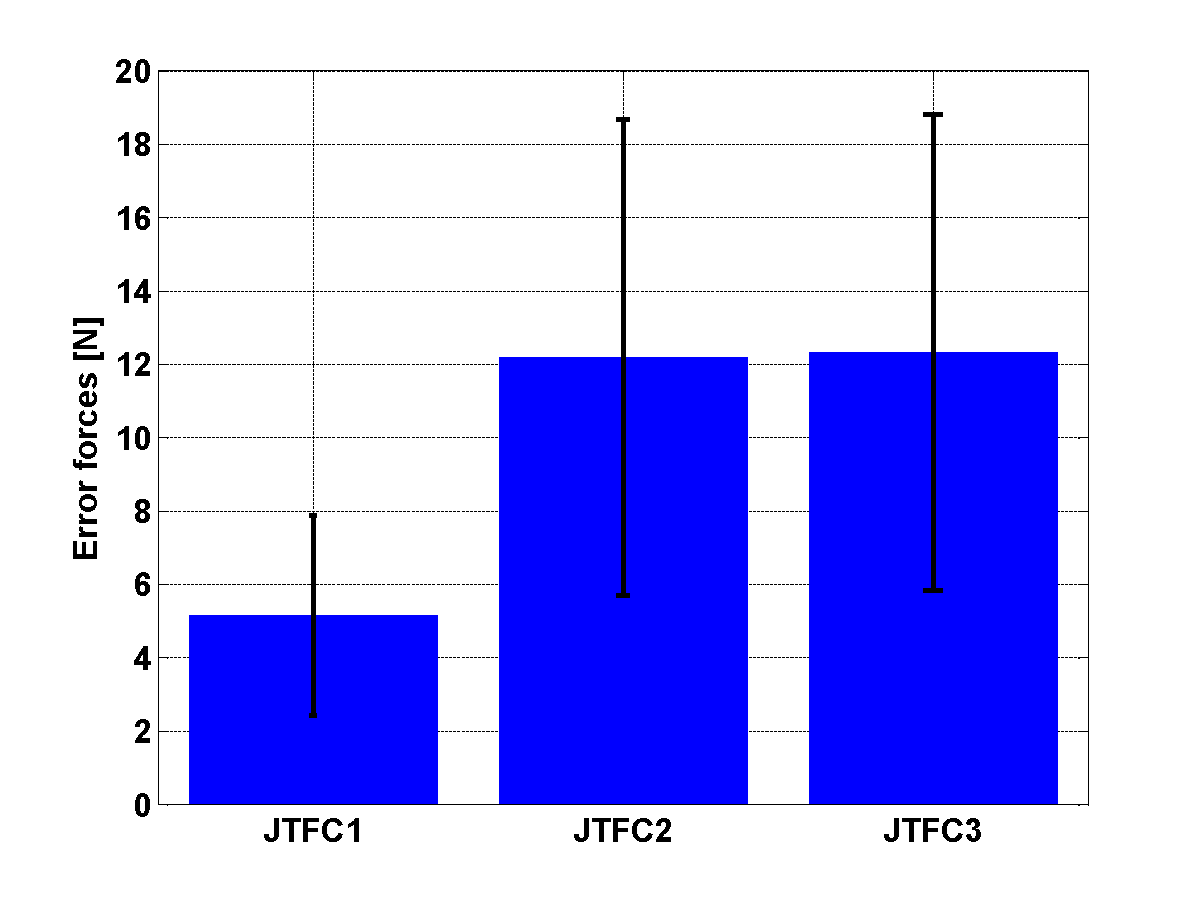
\includegraphics[width=1\columnwidth]{erroreForzaEETrasparenza}
	\def\svgwidth{1\columnwidth}
	\begin{footnotesize}
		\input{imgRevised/transparency_JTFC1_example.pdf_tex}
	\end{footnotesize}
	\caption{An extract of the result of the transparency test using the JTFC1 controller. The user is not hindered by performing a circular trajectory in the XY plane (the z coordinate has a small variation compared to the x and y axis) at constant speed (first row). The
		joint torques (second row) are small compared to the maximum torque that can be exerted by the joints and only the
		$J_3$ torque (the dashed gray line) exhibits a sinusoidal evolution. The third row plot reports the forces measured at the
		end-effector that are always smaller than 25 N.}
	\label{fig:transparencyEeErrors}
\end{figure}
%

\par To complete the transparency analysis, we performed a \emph{smoothness} analysis as proposed in equation 3 of \cite{jarrasse2010methodology}. It is a jerk metric, i.e. the average rate of change of acceleration during a movement. Large values of the smoothness index indicate that many corrections are made during the movement by the subject. 
The values of the smoothness index for the 3 controllers have been reported in \tablename{} \ref{tab:jerkTransparency}.
Differently from the mean torque index, the controller JTFC1 do not exhibit the lowest smoothness value. We suppose this result is related to the less damped behavior performed by the exoskeleton with JTFC1, whereas both JTFC2 and JTFC3 offer a "viscous-like" resistance to the user motion that help smoothing the e.e. trajectory.

\begin{table}[b]
	\renewcommand{\arraystretch}{1.3}
	\caption{Smoothness index for the 3 controllers}
	\label{tab:jerkTransparency}
	\centering
	\begin{tabular}{c c c c}
		\hline \hline
		\bfseries Speed & \bfseries JTFC1 & \bfseries JTFC2 & \bfseries JTFC3 \\
		\hline
		Slow  &  80.87 & 47.10 & 47.80\\ 
		Fast & 107.46  & 85.48 & 119.08 \\
		\hline \hline
	\end{tabular}
\end{table}
%%%%%%%%%%%%%%%%%%%%%%%%%%%%%%%%%%%%%%%%%%%%%%%%%%%%%%%%%%%%%%%%%%%%%%%%%%%%%%%%%%%%%%%%%%%%%%%%%%%%%%%%%%%%%%%%%%%%
%%%%%%%%%%%%%%%%%%%%%%%%%%%%%%%%%%%%%%%%%%%%%%%%%%%%%%%%%%%%%%%%%%%%%%%%%%%%%%%%%%%%%%%%%%%%%%%%%%%%%%%%%%%%%%%%%%%%
\subsection{Haptic rendering}

The implemented torque controls can be used to render the interaction forces exchanged with a virtual surface of a given stiffness and damping, acting as impedance controls. In these tests the contact forces at the end-effector are proportional to the penetration length of the end-effector into the virtual wall surface and to its speed. The force is then converted to desired torques at the joints by multiplying the equation defined in (\ref{eq:desiredVE}) by the transpose of the Jacobian, where the control commands (\ref{eq:JTCF1_control_law_uf_simple}), (\ref{JTFC2_control_law_final}) and (\ref{control_law_Kugi_2} have been used respectively for JFTC1, JFTC2 and JFTC3.
%The design of the exoskeleton allows to control the torque on every joint, so it is possible to render an interaction force not only at the end effector but on every link of the robot. In this case, in equation (\ref{jacobian}) a modified Jacobian will be used to convert forces not applied on the end effector.
\par In the experiments the user grabs the exoskeleton only at the end effector without applying any other force on the links. In this way, the forces measured by the end-effector's force sensor have been used to evaluate the overall system performance since these forces are not involved for the torque control.
\par The rendering experiments were composed by four different type of trials as depicted in \figurename \ \ref{fig:renderingTestType}:
\begin{IEEEdescription}
\item[{\bf T1 }] \hspace{0.5 cm} {\em  "Slide on surface"} experiment with moderate forces;
\item[{\bf T2 }] \hspace{0.5 cm} {\em "Slide on surface" } experiment with high forces;
\item[{\bf T3 }] \hspace{0.5 cm} {\em "Collision with a surface"}  experiment with moderate speed;
\item[{\bf T4 }] \hspace{0.5 cm} {\em "Collision with a surface" } experiment with high speed.
\end{IEEEdescription}

During the T1 and T2 trials the experimenter slided the end-effector on the surface without sudden variations of penetration. The difference between the T1 and T2 trials is the average level of force along the orthogonal axes at the surface.
In the T3 and T4 trials the aim is to test the dynamic performance of the controls, so the experimenter pushed the end-effector on the surface. The difference between the T3 and T4 trials is the average slope of the desired force profiles.
The 4 tests have been evaluated for each controls and with three different environment parameters, in order to consider a low, an intermediate and a high stiff wall. 
\begin{figure}[htb]
	\centering
%	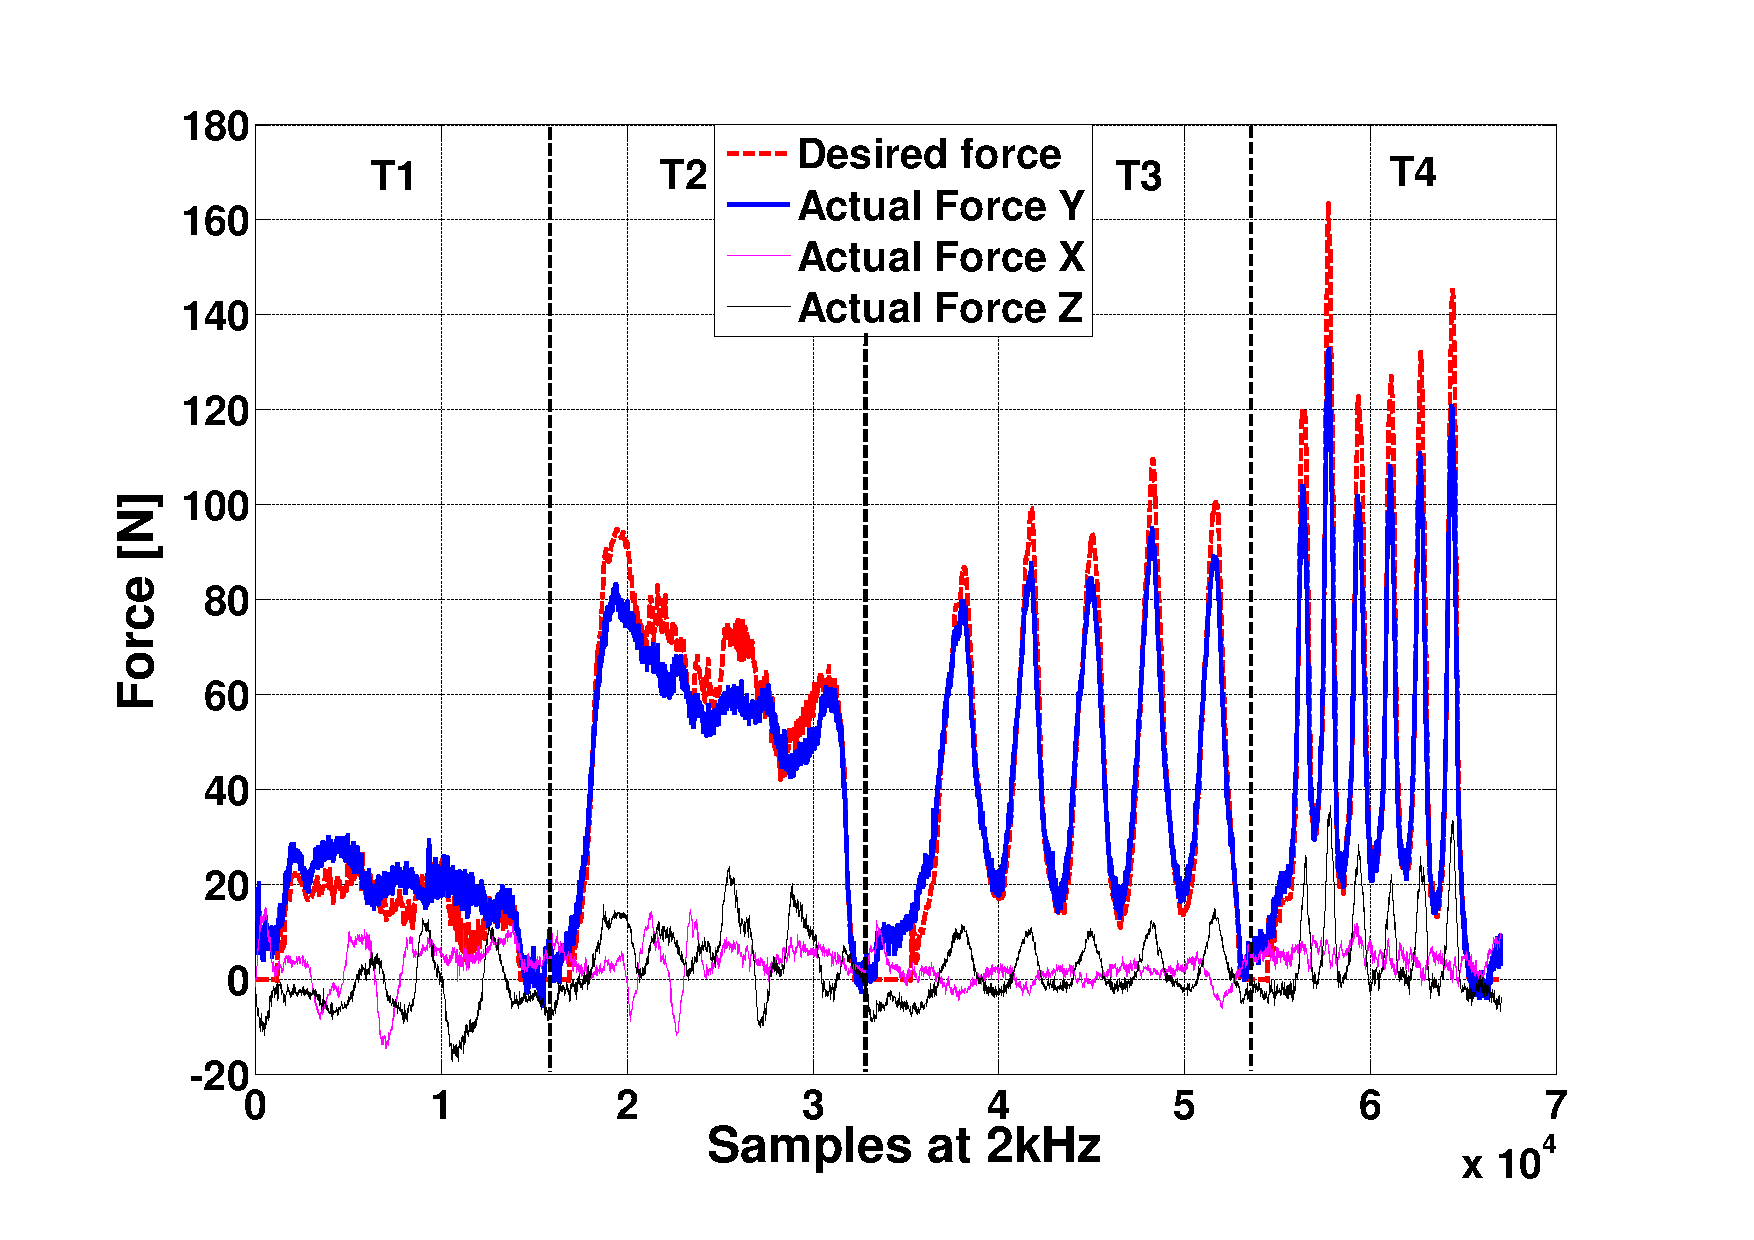
\includegraphics[width=1\columnwidth]{proveRendering}
\def\svgwidth{1\columnwidth}
	\begin{footnotesize}
		\input{imgRevised/hapticTest.pdf_tex}
	\end{footnotesize}
	\caption{The four trial types during an haptic rendering test. The desired forces $F_{y,des}$ are plotted with black solid line whereas the measured orthogonal forces $F_{y,meas}$ are plotted with gray dotted line in the first row. The two tangential components  $F_{x,meas}$ and $F_{z,meas}$ are shown in the second and third rows  respectively.}
	\label{fig:renderingTestType}
\end{figure}

\par The \tablename \ \ref{tab:meanForcesRendering} reports the three environment parameters, the average forces involved in the T1 and T2 trials, the average force peaks and the average slope of the T3 and T4 trials.
%\begin{table}[!t]
%	\renewcommand{\arraystretch}{1.3}
%	\caption{The average forces involved in the T1 and T2 trials, the average force peaks and the average slope of the T3 and T4 trials.}
%	\label{tab:meanForcesRendering}
%	\centering
%	\begin{tabular}{|c|c|c|c|c|}
%		\hline
%		\bfseries Env. Params. & \bfseries T1 & \bfseries T2 & \bfseries T3 & \bfseries T4 \\
%		\hline\hline
%		5 kN/m  &  22.22 $N$ & 50.79 $N$ & 83.33 $N$ & 112.33 $N$\\ 2 Ns/m & - & - & 127.28 $N/s$ & 518.49 $N/s$\\ 
%		\hline
%		20 kN/m &  22.81 $N$ & 66.14 $N$ & 103.97 $N$ & 136.97 $N$\\ 7 Ns/m & - & - & 159.25 $N/s$ & 550.99 $N/s$\\
%		\hline
%		40 kN/m  &  24.98 $N$ & 59.37 $N$ & 88.32 $N$ & 126.20 $N$\\ 10 Ns/m & - & - & 120.39 $N/s$ & 616.03 $N/s$\\
%		\hline
%	\end{tabular}
%\end{table}
\begin{table}[]
	\renewcommand{\arraystretch}{1.3}
	\caption{The average forces involved in the T1 and T2 trials, the average force peaks and the average slope of the T3 and T4 trials.}
	\label{tab:meanForcesRendering}
	\centering
	\begin{tabular}{c c c c c}
		\hline \hline
		\bfseries Env. Params. & \bfseries T1 & \bfseries T2 & \bfseries T3 & \bfseries T4 \\
		\hline
		5 kN/m  &  22.22 $N$ & 50.79 $N$ & 83.33 $N$ & 112.33 $N$\\ 2 Ns/m & - & - & 127.28 $N/s$ & 518.49 $N/s$\\ 
		\hline
		20 kN/m &  22.81 $N$ & 66.14 $N$ & 103.97 $N$ & 136.97 $N$\\ 7 Ns/m & - & - & 159.25 $N/s$ & 550.99 $N/s$\\
		\hline
		40 kN/m  &  24.98 $N$ & 59.37 $N$ & 88.32 $N$ & 126.20 $N$\\ 10 Ns/m & - & - & 120.39 $N/s$ & 616.03 $N/s$\\
		\hline \hline
	\end{tabular}
\end{table}

\par To evaluate the performances of the three different torque controls three indexes have been proposed, i.e. 

\setlength{\IEEEiednormlabelsep}{0.7 cm}
\begin{IEEEitemize}
	\item the mean of the norm of the error force vectors;
	\item the mean of the absolute value of the error of the orthogonal component;
	\item the mean of the angle between the desired forces and the measured ones.
\end{IEEEitemize}

\begin{figure}[htb]
	\centering
%	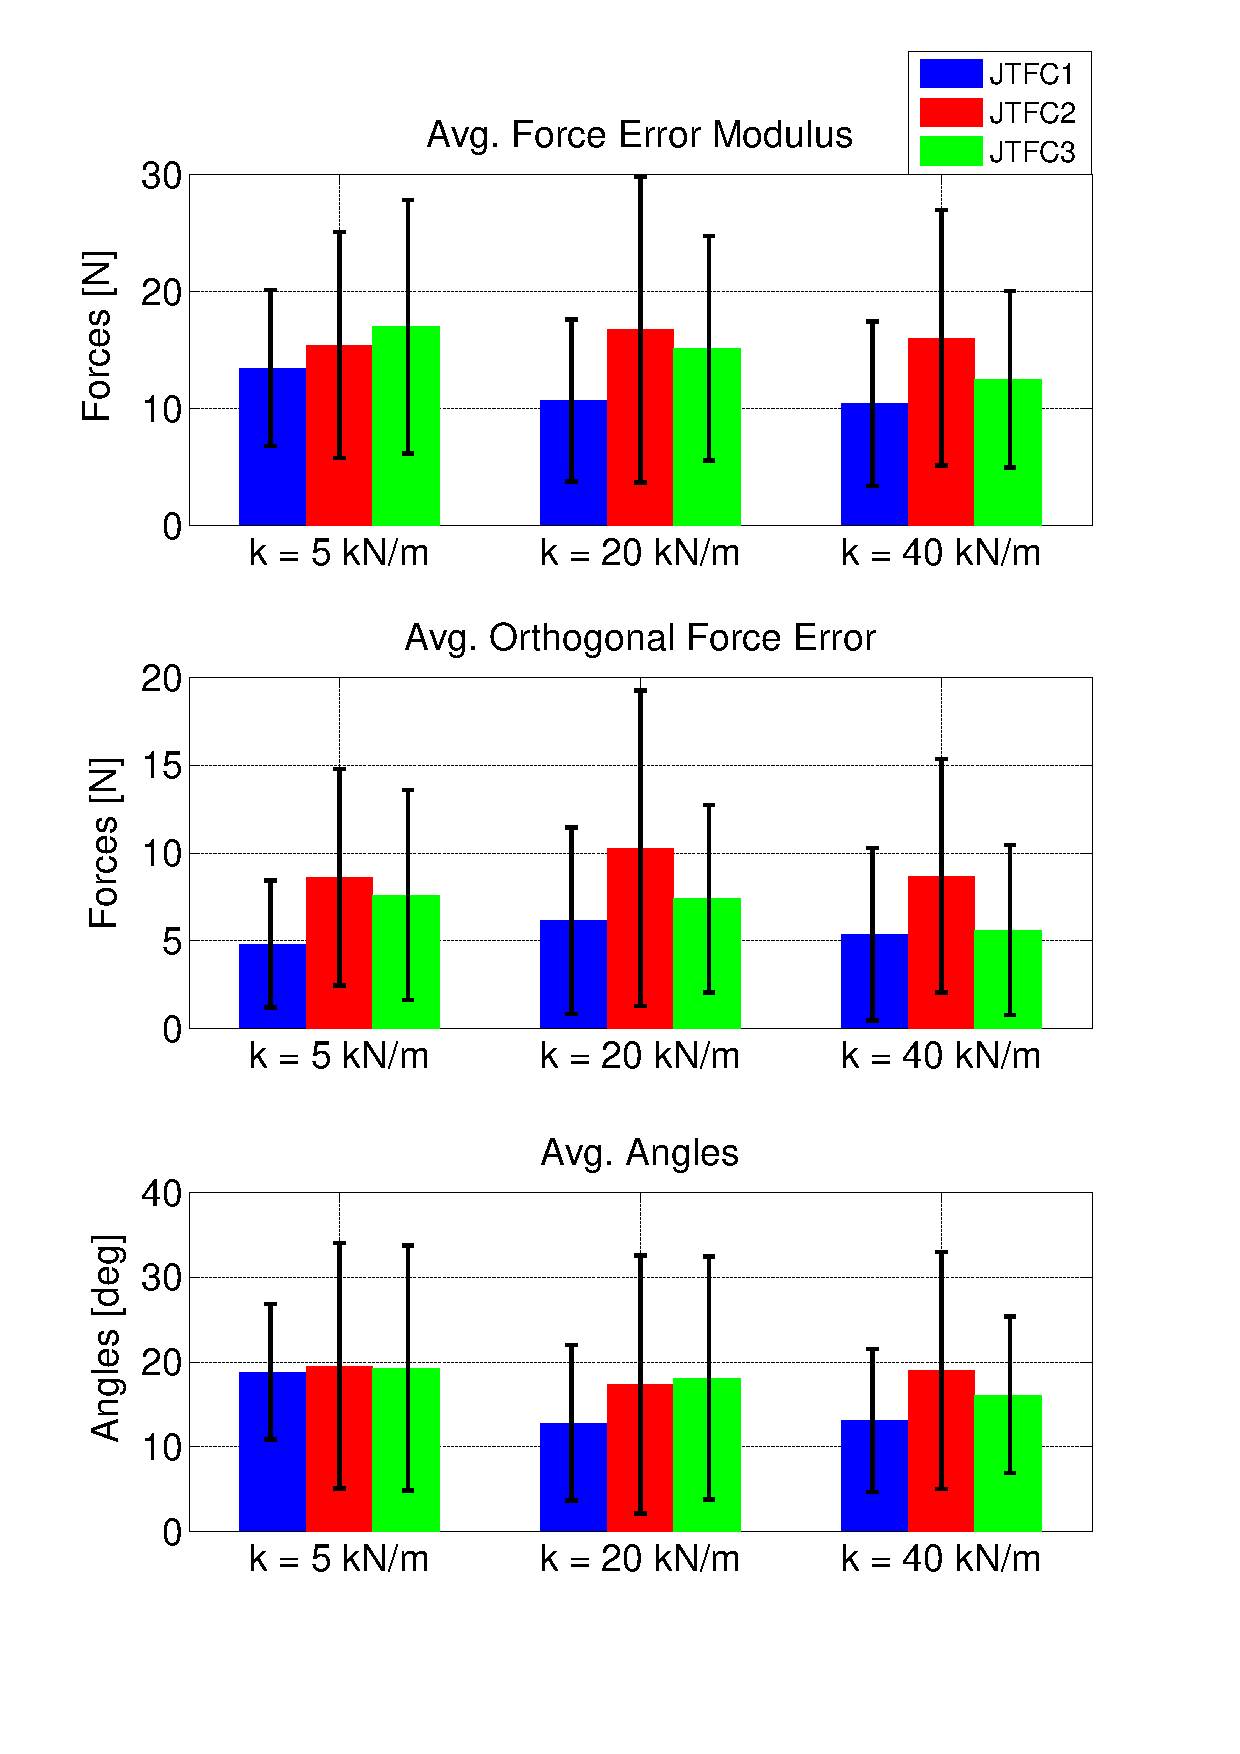
\includegraphics[width=1\columnwidth]{erroriForzeAngoliRendering}
	\def\svgwidth{1\columnwidth}
	\begin{footnotesize}
		\input{imgRevised/hapticRendResults.pdf_tex}
	\end{footnotesize}
	\caption{In the first row, the average of the modulus of the error force vectors at the end effector of the 3 controllers in the rendering task. For this test, 3 stiffness has been evaluated: 5kN/m (small), 20 kN/m (medium) and 40 kN/m (high). In the second row, the average error forces of the orthogonal component. In the third row, the average angle between the desired force vectors and the measured ones.}
	\label{fig:renderingErrors}
\end{figure}

\par The results can be shown in the \figurename \ \ref{fig:renderingErrors}. The first graph shows the average difference between the rendered forces by the controls and the desired forces with an aggregate index, i.e. the norm of the error vector. From this graph the reader can see that in all the condition the JTFC1 control performs better then the others, in fact the mean of the error is around 10 N in all the three cases.
\par To decompose the informations given in the first graph, other two indexes are considered, that are the average error of the orthogonal component of the force and the angle between the desired and the rendered forces. Unlike the norm of the error vector, these two indexes give information on the amplitude and the direction of the undesired force components. The second graph highlights that the JTFC1 control leads to an average error of 5 N along the task direction independently from the environment parameters, that is a good result coupled with the exhibited stable contact with the surface in every condition.
The third graph is substantially in agreement with the previous ones.